% Options for packages loaded elsewhere
\PassOptionsToPackage{unicode}{hyperref}
\PassOptionsToPackage{hyphens}{url}
\PassOptionsToPackage{dvipsnames,svgnames*,x11names*}{xcolor}
%
\documentclass[
  11pt,
]{article}
\usepackage{lmodern}
\usepackage{amsmath}
\usepackage{ifxetex,ifluatex}
\ifnum 0\ifxetex 1\fi\ifluatex 1\fi=0 % if pdftex
  \usepackage[T1]{fontenc}
  \usepackage[utf8]{inputenc}
  \usepackage{textcomp} % provide euro and other symbols
  \usepackage{amssymb}
\else % if luatex or xetex
  \usepackage{unicode-math}
  \defaultfontfeatures{Scale=MatchLowercase}
  \defaultfontfeatures[\rmfamily]{Ligatures=TeX,Scale=1}
  \setmainfont[]{Times New Roman}
\fi
% Use upquote if available, for straight quotes in verbatim environments
\IfFileExists{upquote.sty}{\usepackage{upquote}}{}
\IfFileExists{microtype.sty}{% use microtype if available
  \usepackage[]{microtype}
  \UseMicrotypeSet[protrusion]{basicmath} % disable protrusion for tt fonts
}{}
\usepackage{xcolor}
\IfFileExists{xurl.sty}{\usepackage{xurl}}{} % add URL line breaks if available
\IfFileExists{bookmark.sty}{\usepackage{bookmark}}{\usepackage{hyperref}}
\hypersetup{
  colorlinks=true,
  linkcolor=black,
  filecolor=Maroon,
  citecolor=Blue,
  urlcolor=Blue,
  pdfcreator={LaTeX via pandoc}}
\urlstyle{same} % disable monospaced font for URLs
\usepackage[margin=1in]{geometry}
\usepackage{longtable,booktabs}
\usepackage{calc} % for calculating minipage widths
% Correct order of tables after \paragraph or \subparagraph
\usepackage{etoolbox}
\makeatletter
\patchcmd\longtable{\par}{\if@noskipsec\mbox{}\fi\par}{}{}
\makeatother
% Allow footnotes in longtable head/foot
\IfFileExists{footnotehyper.sty}{\usepackage{footnotehyper}}{\usepackage{footnote}}
\makesavenoteenv{longtable}
\usepackage{graphicx}
\makeatletter
\def\maxwidth{\ifdim\Gin@nat@width>\linewidth\linewidth\else\Gin@nat@width\fi}
\def\maxheight{\ifdim\Gin@nat@height>\textheight\textheight\else\Gin@nat@height\fi}
\makeatother
% Scale images if necessary, so that they will not overflow the page
% margins by default, and it is still possible to overwrite the defaults
% using explicit options in \includegraphics[width, height, ...]{}
\setkeys{Gin}{width=\maxwidth,height=\maxheight,keepaspectratio}
% Set default figure placement to htbp
\makeatletter
\def\fps@figure{htbp}
\makeatother
\setlength{\emergencystretch}{3em} % prevent overfull lines
\providecommand{\tightlist}{%
  \setlength{\itemsep}{0pt}\setlength{\parskip}{0pt}}
\setcounter{secnumdepth}{-\maxdimen} % remove section numbering
\usepackage{booktabs}
\usepackage{longtable}
\usepackage{array}
\usepackage{multirow}
\usepackage{wrapfig}
\usepackage{float}
\usepackage{colortbl}
\usepackage{pdflscape}
\usepackage{tabu}
\usepackage{threeparttable}
\usepackage{threeparttablex}
\usepackage[normalem]{ulem}
\usepackage{makecell}
\usepackage{xcolor}
\usepackage{fontspec}
\usepackage{multicol}
\usepackage{hhline}
\usepackage{hyperref}
\usepackage{caption}
\usepackage{graphicx}
\usepackage{siunitx}
\usepackage{calc}
\usepackage{tabularx}
\usepackage{adjustbox}
\ifluatex
  \usepackage{selnolig}  % disable illegal ligatures
\fi
\newlength{\cslhangindent}
\setlength{\cslhangindent}{1.5em}
\newlength{\csllabelwidth}
\setlength{\csllabelwidth}{3em}
\newenvironment{CSLReferences}[2] % #1 hanging-ident, #2 entry spacing
 {% don't indent paragraphs
  \setlength{\parindent}{0pt}
  % turn on hanging indent if param 1 is 1
  \ifodd #1 \everypar{\setlength{\hangindent}{\cslhangindent}}\ignorespaces\fi
  % set entry spacing
  \ifnum #2 > 0
  \setlength{\parskip}{#2\baselineskip}
  \fi
 }%
 {}
\usepackage{calc}
\newcommand{\CSLBlock}[1]{#1\hfill\break}
\newcommand{\CSLLeftMargin}[1]{\parbox[t]{\csllabelwidth}{#1}}
\newcommand{\CSLRightInline}[1]{\parbox[t]{\linewidth - \csllabelwidth}{#1}\break}
\newcommand{\CSLIndent}[1]{\hspace{\cslhangindent}#1}

\author{}
\date{\vspace{-2.5em}}

\begin{document}

\hypertarget{introduction}{%
\section{Introduction}\label{introduction}}

The policy environment for Lesbian, Gay, and Bisexual (LGB) couples around the world has changed rapidly in recent years. One notable shift is the 2013 U.S. Supreme Court decision ruling the Defense of Marriage Act (DOMA) unconstitutional. For the first time, U.S. citizens could sponsor the visa of their same-sex spouse. Redpath (2022) demonstrates that end of DOMA resulted in a significant increase in unions between mixed-citizenship, same-sex couples. However, as show in Figure \ref{fig:desc}, this rapid increase after 2013 was not uniform across immigrants from all countries. For those hailing from countries with progressive LGB policies, the increase was indeed rapid after 2013. However, from those with repressive LGB policies, no increase occurred.

Using waves 2008 to 2019 of the American Community Survey, this study employs a difference-in-differences-in-differences (DDD) design to examine how the policy environment of the origin country moderates the effect of the end of DOMA on the incidence of same-sex, mixed-citizenship couples into unions. Using quasi-Poisson models with two-way fixed effects, we show that, after 2013, individuals in mixed-citizenship, same-sex couples hailing from countries with progressive LGB policy saw a more than 50-percent increase in incidence relative to those in different-sex or same-citizenship couples. Meanwhile, those from countries with repressive laws experienced no relative increase at all. We argue that the policy context of country of origin leaves a lasting cultural impact on immigrants that shapes their response to policy shifts in their country of residence, even many years after migration.

\begin{figure}
\centering
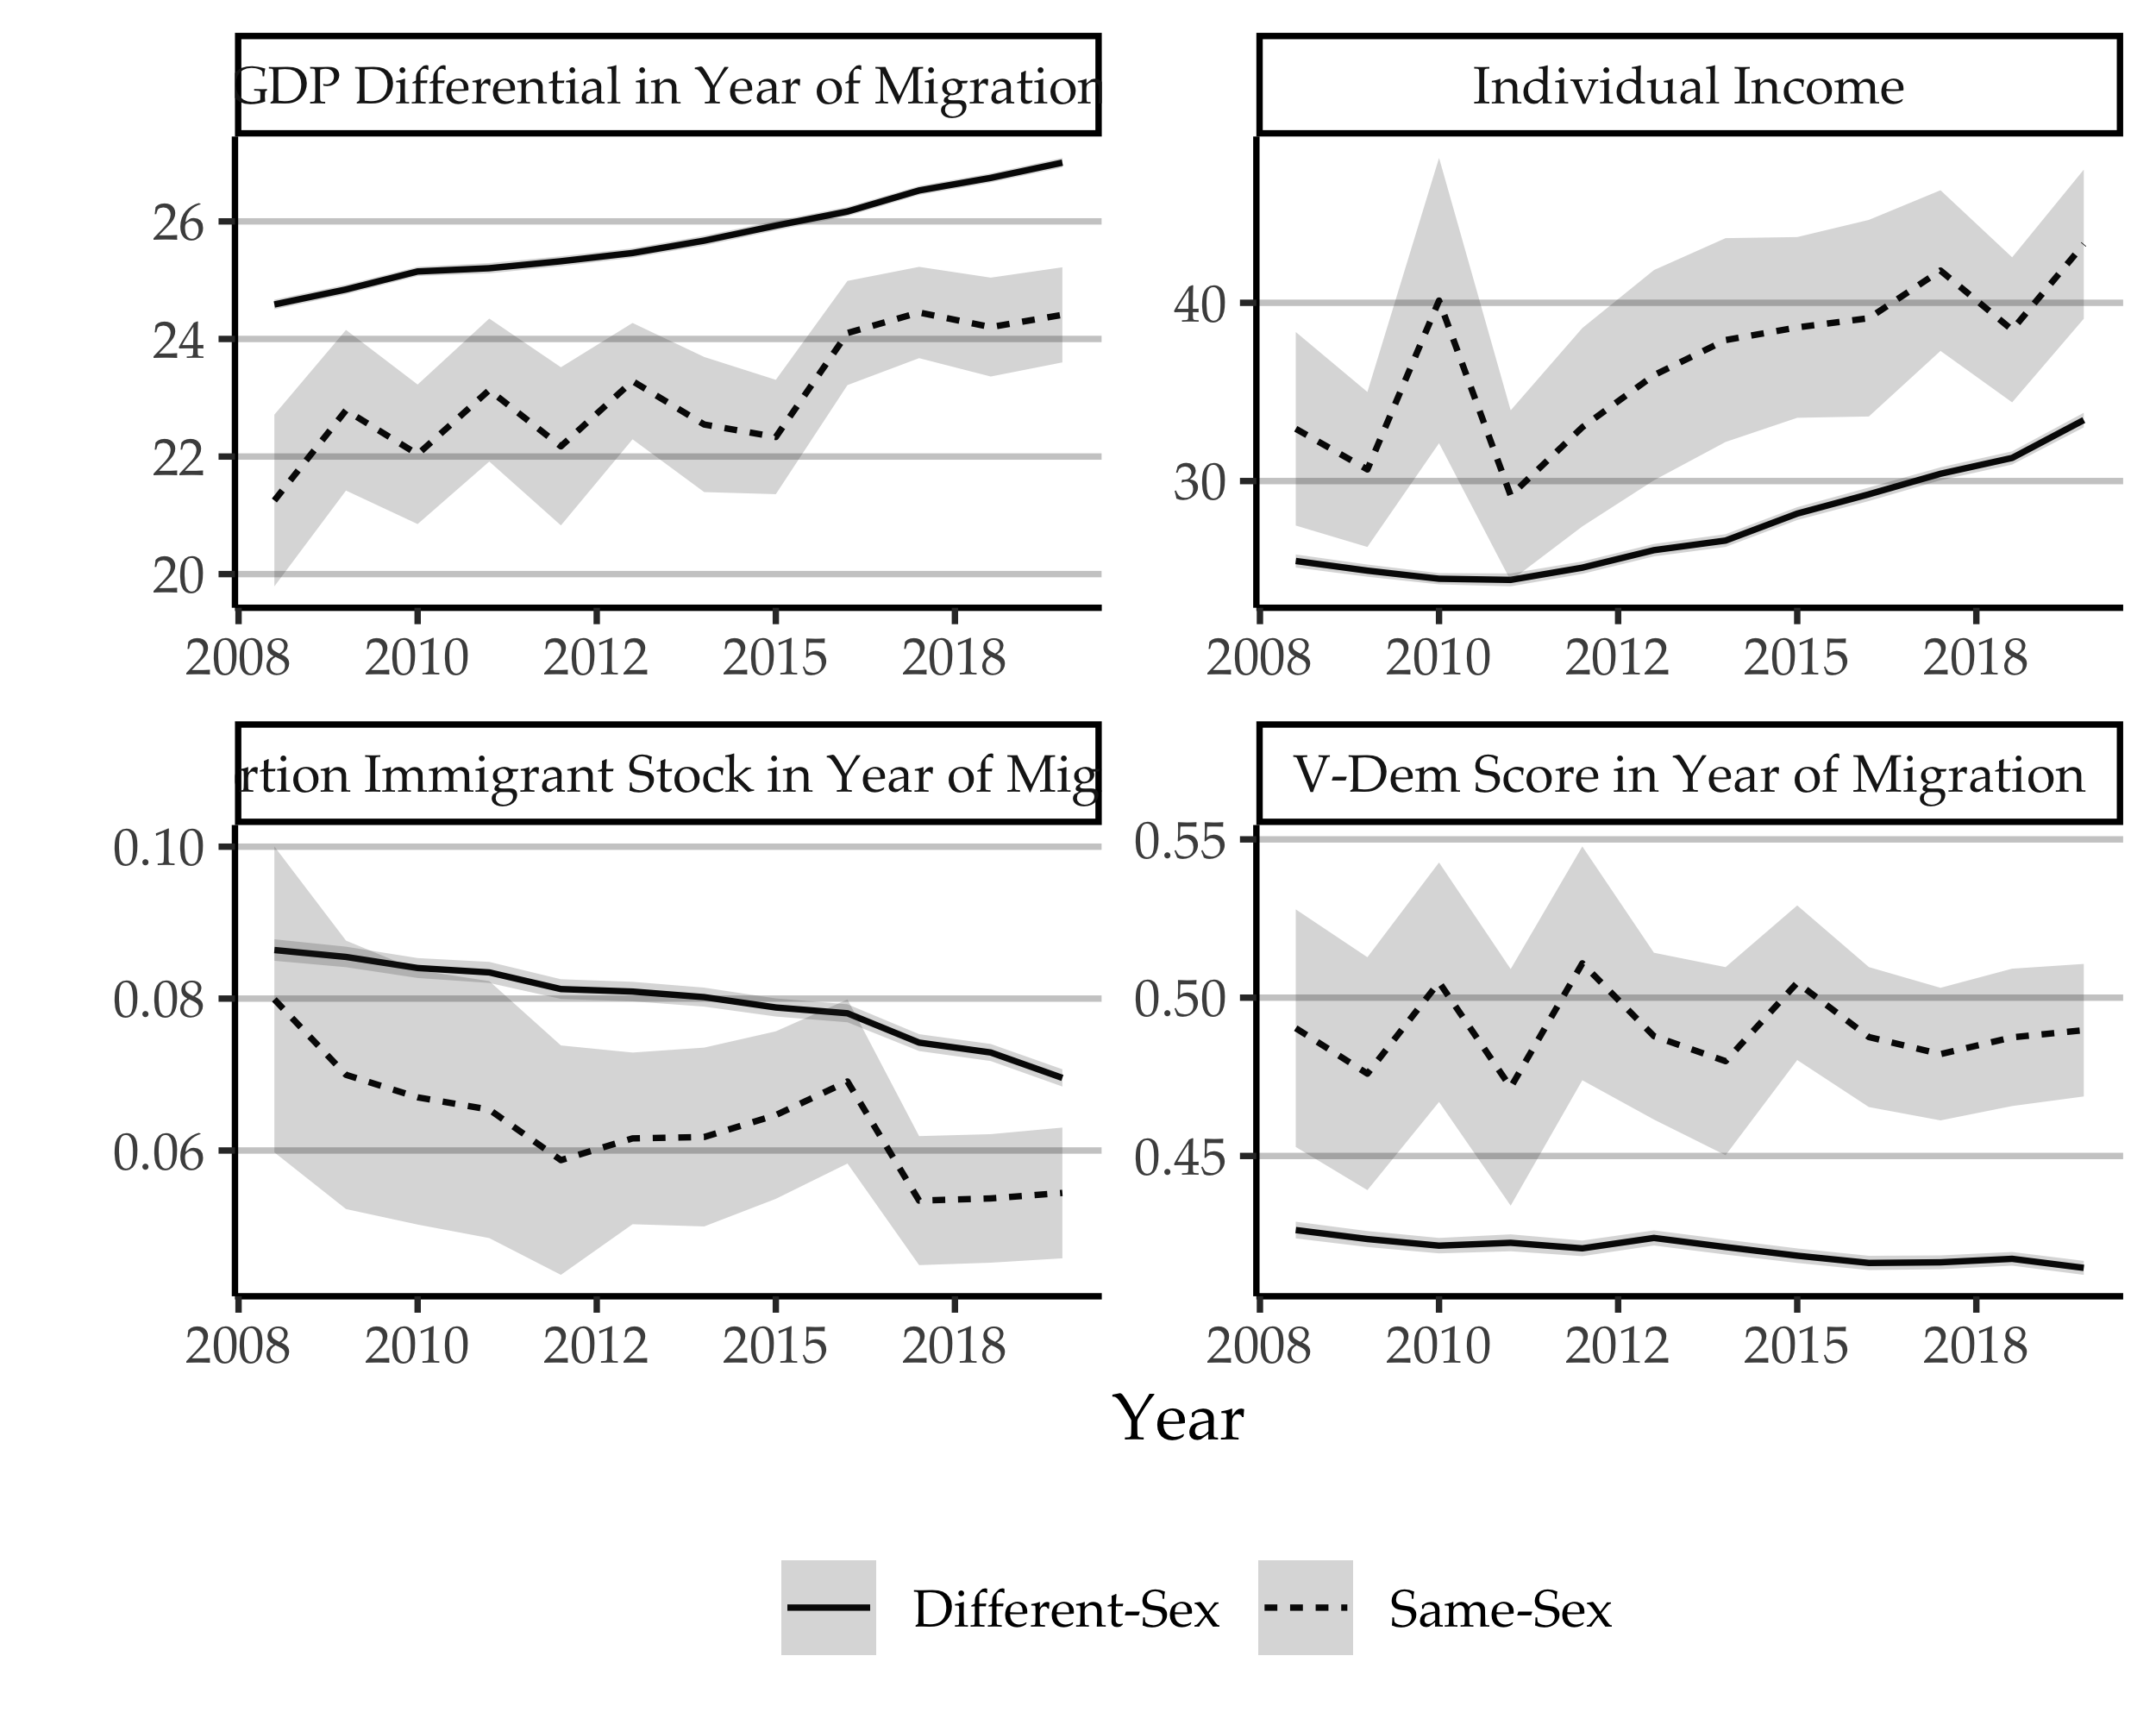
\includegraphics{asa_ssimm_did_files/figure-latex/desc-1.pdf}
\caption{\label{fig:desc}Estimated counts of individuals in mixed-citizenship, same-same couples from the American Community Survey. The ``Repressive'' sample includes only countries with a LGB policy score less than 0, and the ``Progressive'' sample includes only those with a score greater than 3.}
\end{figure}

\hypertarget{research-questions}{%
\section{Research Questions}\label{research-questions}}

\begin{enumerate}
\def\labelenumi{\arabic{enumi}.}
\item
  How does LGB policy at country of origin moderate the effect of the repeal of DOMA on the incidence of same-sex, mixed-citizenship couples in the U.S.?
\item
  Which specific LGB policies of country of origin are most relevant in shaping entry into same-sex unions?
\end{enumerate}

\hypertarget{background}{%
\section{Background}\label{background}}

The United States Supreme Court overturned the Defense of Marriage Act (DOMA) in United States v. Windsor in 2013. Enacted in 1996, DOMA banned the federal government from recognizing same-sex marriages. The Windsor decision carried significant implications for same-sex couples. Most relevantly for this paper, it unlocked spousal visas for same-sex couples. As a direct consequence of undoing DOMA, Redpath (2022) finds a 36 percent relative increase in spousal visas for mixed-citizen couples and a 78 percent increase in mixed-citizen marriages.

Although the DOMA decision equally applied to all mixed-citizenship couples, Figure \ref{fig:desc} highlights an important line of differentiation: there is a distinct rise in couples where the non-U.S. citizen came from a country with more progressive LGB policies. Couples where the non-U.S. citizen came from a country with repressive LGB policies, such as bans on sodomy, remain unchanged. Why might this be? Why would conditions at the immigrant partner's country of origin influence the distribution of same-sex union formation across the population of mixed-citizen couples within the U.S.? We argue that by investigating the interplay between law and culture, we can understand the discrepancies found in Figure 1.

Relationships, and marriage specifically, are unique cultural products. The rituals, symbols, norms, and roles that govern them have different instantiations depending on the time and place. These cultural products then influence and are influenced by the legal expectations and conditions associated with relationships. This is especially true for same-sex unions in the present historical moment; assimilation of same-sex couples into existing marriage and relationship programs is a very current, dynamic process.

One important consequence of these shifts is that they change our understanding of what it permissible and seen as possible. Prior to state recognition, there are often public campaigns by LGBT+ organizers seeking to influence broad support, which helps socialize LGB individuals into the appropriateness of participating in these institutions. This is particularly important as participation in same-sex unions by LGB individuals is a critical strategy to normalize and secure such legal advancements. State recognition of same-sex couples also takes on a recursive process of increasing desirability of forming such a union as participation becomes a real option. Thus, immigrants coming from a country with an affirming policy environment that recognizes the validity of same-sex unions may be more inclined to establish and desire such a union once permitted to do so following DOMA.

Conversely, policy environments that are especially repressive can hinder the formation of mixed-citizenship, same-sex unions by immigrants in the U.S. This can operate in multiple ways. First, repressive contexts can potentially limit the desirability of forming a same-sex union by limiting what is seen as possible. At the end of 2021, roughly 70 countries still criminalized same-sex sexual acts between two consenting adults. Moreover, more than 30 countries since the 1990s have re-codified a ``one man, one woman'' definition of marriage either through federal law like DOMA or through constitutional amendments. Second, these legal environments can influence how the cultural norms, rituals, and performances of relationships manifest. Where marriage equality exists, mainstream LGB cultures emphasize publicly ``coming out'' and sameness with heterosexuals using language such as ``love is love.'' But LGB cultures where ``coming out'' risks vulnerability to state-sponsored violence can look quite different. Third, and relatedly, these different cultures can negatively influence whether U.S. immigration bureaucrats in charge of issuing visas perceive relationships as legitimate. When photos, disclosure to friends and family, and other public pieces of evidence are used to evaluate if a relationship is valid and worthy of a visa, immigrants coming from countries where such pieces of evidence can be harmful are at a systematic disadvantage. Thus, for all of these reasons, mixed-citizen, same-sex unions following the 2013 DOMA decision are likely to contain fewer immigrant partners from repressive contexts.

\hypertarget{data-and-methods}{%
\section{Data and Methods}\label{data-and-methods}}

We employ data from the 2008 to 2019 American Community Survey. Each year, the ACS surveys a 1-percent representative sample of the U.S. population about a variety of individual and household attributes. We focus on counts of individuals in mixed-citizenship same-sex couples, comparing to those in same-citizenship or different-sex couples. Our counts include only cohabiting individuals who identify themselves as spouses or unmarried partners, since the ACS does not allow identification of same-sex couples that do not reside together. ``Mixed-citizenship'' couples include either two citizens or two non-citizens, and ``same-sex'' couples include two individuals who report the same sex. We exclude individuals who immigrated before the age of 18 as well as those younger than 18 or older than 64 in each survey year.

Beginning in 2008 the Census Bureau made changes to ACS gender and partnership questions in order to prevent such errors, so we rely on data only from 2008 onward. In addition, following previous research, we remove all respondents that had either their relationship or sex variable imputed by the Census Bureau. See Table \ref{tab:data-tab} for sample sizes.

\providecommand{\docline}[3]{\noalign{\global\setlength{\arrayrulewidth}{#1}}\arrayrulecolor[HTML]{#2}\cline{#3}}

\setlength{\tabcolsep}{2pt}

\renewcommand*{\arraystretch}{1.5}

\begin{longtable}[c]{|p{0.88in}|p{1.40in}|p{1.21in}|p{1.16in}}

\caption{Unweighted and weighted sample sizes from American Community Survey (ACS) data, 2008-2019}\label{tab:data-tab}\\

\hhline{>{\arrayrulecolor[HTML]{666666}\global\arrayrulewidth=2pt}->{\arrayrulecolor[HTML]{666666}\global\arrayrulewidth=2pt}->{\arrayrulecolor[HTML]{666666}\global\arrayrulewidth=2pt}->{\arrayrulecolor[HTML]{666666}\global\arrayrulewidth=2pt}-}

\multicolumn{1}{!{\color[HTML]{000000}\vrule width 0pt}>{\raggedleft}p{\dimexpr 0.88in+0\tabcolsep+0\arrayrulewidth}}{\fontsize{11}{11}\selectfont{\textcolor[HTML]{000000}{\global\setmainfont{Times New Roman}{Same-sex}}}} & \multicolumn{1}{!{\color[HTML]{000000}\vrule width 0pt}>{\raggedleft}p{\dimexpr 1.4in+0\tabcolsep+0\arrayrulewidth}}{\fontsize{11}{11}\selectfont{\textcolor[HTML]{000000}{\global\setmainfont{Times New Roman}{Mixed-citizenship}}}} & \multicolumn{1}{!{\color[HTML]{000000}\vrule width 0pt}>{\raggedleft}p{\dimexpr 1.21in+0\tabcolsep+0\arrayrulewidth}}{\fontsize{11}{11}\selectfont{\textcolor[HTML]{000000}{\global\setmainfont{Times New Roman}{n\ (unweighted)}}}} & \multicolumn{1}{!{\color[HTML]{000000}\vrule width 0pt}>{\raggedleft}p{\dimexpr 1.16in+0\tabcolsep+0\arrayrulewidth}!{\color[HTML]{000000}\vrule width 0pt}}{\fontsize{11}{11}\selectfont{\textcolor[HTML]{000000}{\global\setmainfont{Times New Roman}{n\ (weighted)}}}} \\

\noalign{\global\setlength{\arrayrulewidth}{2pt}}\arrayrulecolor[HTML]{666666}\cline{1-4}

\endfirsthead

\hhline{>{\arrayrulecolor[HTML]{666666}\global\arrayrulewidth=2pt}->{\arrayrulecolor[HTML]{666666}\global\arrayrulewidth=2pt}->{\arrayrulecolor[HTML]{666666}\global\arrayrulewidth=2pt}->{\arrayrulecolor[HTML]{666666}\global\arrayrulewidth=2pt}-}

\multicolumn{1}{!{\color[HTML]{000000}\vrule width 0pt}>{\raggedleft}p{\dimexpr 0.88in+0\tabcolsep+0\arrayrulewidth}}{\fontsize{11}{11}\selectfont{\textcolor[HTML]{000000}{\global\setmainfont{Times New Roman}{Same-sex}}}} & \multicolumn{1}{!{\color[HTML]{000000}\vrule width 0pt}>{\raggedleft}p{\dimexpr 1.4in+0\tabcolsep+0\arrayrulewidth}}{\fontsize{11}{11}\selectfont{\textcolor[HTML]{000000}{\global\setmainfont{Times New Roman}{Mixed-citizenship}}}} & \multicolumn{1}{!{\color[HTML]{000000}\vrule width 0pt}>{\raggedleft}p{\dimexpr 1.21in+0\tabcolsep+0\arrayrulewidth}}{\fontsize{11}{11}\selectfont{\textcolor[HTML]{000000}{\global\setmainfont{Times New Roman}{n\ (unweighted)}}}} & \multicolumn{1}{!{\color[HTML]{000000}\vrule width 0pt}>{\raggedleft}p{\dimexpr 1.16in+0\tabcolsep+0\arrayrulewidth}!{\color[HTML]{000000}\vrule width 0pt}}{\fontsize{11}{11}\selectfont{\textcolor[HTML]{000000}{\global\setmainfont{Times New Roman}{n\ (weighted)}}}} \\

\noalign{\global\setlength{\arrayrulewidth}{2pt}}\arrayrulecolor[HTML]{666666}\cline{1-4}\endhead



\multicolumn{1}{!{\color[HTML]{000000}\vrule width 0pt}>{\raggedleft}p{\dimexpr 0.88in+0\tabcolsep+0\arrayrulewidth}}{\fontsize{11}{11}\selectfont{\textcolor[HTML]{000000}{\global\setmainfont{Times New Roman}{FALSE}}}} & \multicolumn{1}{!{\color[HTML]{000000}\vrule width 0pt}>{\raggedleft}p{\dimexpr 1.4in+0\tabcolsep+0\arrayrulewidth}}{\fontsize{11}{11}\selectfont{\textcolor[HTML]{000000}{\global\setmainfont{Times New Roman}{FALSE}}}} & \multicolumn{1}{!{\color[HTML]{000000}\vrule width 0pt}>{\raggedleft}p{\dimexpr 1.21in+0\tabcolsep+0\arrayrulewidth}}{\fontsize{11}{11}\selectfont{\textcolor[HTML]{000000}{\global\setmainfont{Times New Roman}{11,103,024}}}} & \multicolumn{1}{!{\color[HTML]{000000}\vrule width 0pt}>{\raggedleft}p{\dimexpr 1.16in+0\tabcolsep+0\arrayrulewidth}!{\color[HTML]{000000}\vrule width 0pt}}{\fontsize{11}{11}\selectfont{\textcolor[HTML]{000000}{\global\setmainfont{Times New Roman}{1,046,422,984}}}} \\





\multicolumn{1}{!{\color[HTML]{000000}\vrule width 0pt}>{\raggedleft}p{\dimexpr 0.88in+0\tabcolsep+0\arrayrulewidth}}{\fontsize{11}{11}\selectfont{\textcolor[HTML]{000000}{\global\setmainfont{Times New Roman}{FALSE}}}} & \multicolumn{1}{!{\color[HTML]{000000}\vrule width 0pt}>{\raggedleft}p{\dimexpr 1.4in+0\tabcolsep+0\arrayrulewidth}}{\fontsize{11}{11}\selectfont{\textcolor[HTML]{000000}{\global\setmainfont{Times New Roman}{TRUE}}}} & \multicolumn{1}{!{\color[HTML]{000000}\vrule width 0pt}>{\raggedleft}p{\dimexpr 1.21in+0\tabcolsep+0\arrayrulewidth}}{\fontsize{11}{11}\selectfont{\textcolor[HTML]{000000}{\global\setmainfont{Times New Roman}{467,611}}}} & \multicolumn{1}{!{\color[HTML]{000000}\vrule width 0pt}>{\raggedleft}p{\dimexpr 1.16in+0\tabcolsep+0\arrayrulewidth}!{\color[HTML]{000000}\vrule width 0pt}}{\fontsize{11}{11}\selectfont{\textcolor[HTML]{000000}{\global\setmainfont{Times New Roman}{50,313,621}}}} \\





\multicolumn{1}{!{\color[HTML]{000000}\vrule width 0pt}>{\raggedleft}p{\dimexpr 0.88in+0\tabcolsep+0\arrayrulewidth}}{\fontsize{11}{11}\selectfont{\textcolor[HTML]{000000}{\global\setmainfont{Times New Roman}{TRUE}}}} & \multicolumn{1}{!{\color[HTML]{000000}\vrule width 0pt}>{\raggedleft}p{\dimexpr 1.4in+0\tabcolsep+0\arrayrulewidth}}{\fontsize{11}{11}\selectfont{\textcolor[HTML]{000000}{\global\setmainfont{Times New Roman}{FALSE}}}} & \multicolumn{1}{!{\color[HTML]{000000}\vrule width 0pt}>{\raggedleft}p{\dimexpr 1.21in+0\tabcolsep+0\arrayrulewidth}}{\fontsize{11}{11}\selectfont{\textcolor[HTML]{000000}{\global\setmainfont{Times New Roman}{147,459}}}} & \multicolumn{1}{!{\color[HTML]{000000}\vrule width 0pt}>{\raggedleft}p{\dimexpr 1.16in+0\tabcolsep+0\arrayrulewidth}!{\color[HTML]{000000}\vrule width 0pt}}{\fontsize{11}{11}\selectfont{\textcolor[HTML]{000000}{\global\setmainfont{Times New Roman}{13,630,989}}}} \\





\multicolumn{1}{!{\color[HTML]{000000}\vrule width 0pt}>{\raggedleft}p{\dimexpr 0.88in+0\tabcolsep+0\arrayrulewidth}}{\fontsize{11}{11}\selectfont{\textcolor[HTML]{000000}{\global\setmainfont{Times New Roman}{TRUE}}}} & \multicolumn{1}{!{\color[HTML]{000000}\vrule width 0pt}>{\raggedleft}p{\dimexpr 1.4in+0\tabcolsep+0\arrayrulewidth}}{\fontsize{11}{11}\selectfont{\textcolor[HTML]{000000}{\global\setmainfont{Times New Roman}{TRUE}}}} & \multicolumn{1}{!{\color[HTML]{000000}\vrule width 0pt}>{\raggedleft}p{\dimexpr 1.21in+0\tabcolsep+0\arrayrulewidth}}{\fontsize{11}{11}\selectfont{\textcolor[HTML]{000000}{\global\setmainfont{Times New Roman}{7,305}}}} & \multicolumn{1}{!{\color[HTML]{000000}\vrule width 0pt}>{\raggedleft}p{\dimexpr 1.16in+0\tabcolsep+0\arrayrulewidth}!{\color[HTML]{000000}\vrule width 0pt}}{\fontsize{11}{11}\selectfont{\textcolor[HTML]{000000}{\global\setmainfont{Times New Roman}{694,122}}}} \\

\noalign{\global\setlength{\arrayrulewidth}{2pt}}\arrayrulecolor[HTML]{666666}\cline{1-4}



\end{longtable}

To isolate the effect of the 2013 DOMA repeal, we employ a difference-in-differences-in-differences (DDD) Poisson design. We model counts as draws from a Poisson distribution, but estimate our model more flexibly by using quasi-maximum likelihood estimation (QMLE). Unlike Maximum Likelihood Estimation (MLE), this estimation method does not assume the mean and variance of the distribution are equal, adjusting standard errors accordingly. We include two-way fixed effects, with indicators for survey year and state-group, and cluster standard errors at the state-group level.

Our estimand is the relative change in incidence of individual in mixed-citizenship, same-sex couples following the repeal of DOMA in 2013. We estimate this as the coefficient to a three-way interaction between indicators for same-sex, mixed-citizenship, and post-2013 survey year. We focus on heterogeneity of this effect: how it varies by the LGB policy context of non-citizens' country of origin. We measure the origin country policy environment using an LGB Policy Index for 1991 to 2019. The index is created by summing the net total of progressive policies (scored \(+1\)) over regressive policies (scored \(-1\)). The country index ranges from -3 to 10, with a mean of 1.7 in our sample. Group-state-year-country cells are assigned the average score in the year of immigration for non-citizen individuals in that cell.

\hypertarget{preliminary-results}{%
\section{Preliminary Results}\label{preliminary-results}}

 
  \providecommand{\huxb}[2]{\arrayrulecolor[RGB]{#1}\global\arrayrulewidth=#2pt}
  \providecommand{\huxvb}[2]{\color[RGB]{#1}\vrule width #2pt}
  \providecommand{\huxtpad}[1]{\rule{0pt}{#1}}
  \providecommand{\huxbpad}[1]{\rule[-#1]{0pt}{#1}}

\begin{table}[ht]
\begin{centerbox}
\begin{threeparttable}
\captionsetup{justification=centering,singlelinecheck=off}
\caption{\label{tab:mod-tab} Quasi-Poisson DDD regressions of counts of 
                        mixed-citizenship same-sex couples}
 \setlength{\tabcolsep}{0pt}
\begin{tabularx}{1\textwidth}{p{0.25\textwidth} p{0.25\textwidth} p{0.25\textwidth} p{0.25\textwidth}}


\hhline{>{\huxb{0, 0, 0}{0.8}}->{\huxb{0, 0, 0}{0.8}}->{\huxb{0, 0, 0}{0.8}}->{\huxb{0, 0, 0}{0.8}}-}
\arrayrulecolor{black}

\multicolumn{1}{!{\huxvb{0, 0, 0}{0}}p{0.25\textwidth}!{\huxvb{0, 0, 0}{0}}}{\hspace{0pt}\parbox[b]{0.25\textwidth-0pt-0pt}{\huxtpad{0pt + 1em}\centering \huxbpad{0pt}}} &
\multicolumn{1}{p{0.25\textwidth}!{\huxvb{0, 0, 0}{0}}}{\hspace{0pt}\parbox[b]{0.25\textwidth-0pt-0pt}{\huxtpad{0pt + 1em}\centering Full sample\huxbpad{0pt}}} &
\multicolumn{1}{p{0.25\textwidth}!{\huxvb{0, 0, 0}{0}}}{\hspace{0pt}\parbox[b]{0.25\textwidth-0pt-0pt}{\huxtpad{0pt + 1em}\centering Progressive\huxbpad{0pt}}} &
\multicolumn{1}{p{0.25\textwidth}!{\huxvb{0, 0, 0}{0}}}{\hspace{0pt}\parbox[b]{0.25\textwidth-0pt-0pt}{\huxtpad{0pt + 1em}\centering Repressive\huxbpad{0pt}}} \tabularnewline[-0.5pt]


\hhline{>{\huxb{255, 255, 255}{0.4}}->{\huxb{0, 0, 0}{0.4}}->{\huxb{0, 0, 0}{0.4}}->{\huxb{0, 0, 0}{0.4}}-}
\arrayrulecolor{black}

\multicolumn{1}{!{\huxvb{0, 0, 0}{0}}p{0.25\textwidth}!{\huxvb{0, 0, 0}{0}}}{\hspace{0pt}\parbox[b]{0.25\textwidth-0pt-0pt}{\huxtpad{0pt + 1em}\raggedright Post-2013 × Same-sex × Mixed-citizenship\huxbpad{0pt}}} &
\multicolumn{1}{p{0.25\textwidth}!{\huxvb{0, 0, 0}{0}}}{\hspace{0pt}\parbox[b]{0.25\textwidth-0pt-0pt}{\huxtpad{0pt + 1em}\raggedleft 0.326 ***\huxbpad{0pt}}} &
\multicolumn{1}{p{0.25\textwidth}!{\huxvb{0, 0, 0}{0}}}{\hspace{0pt}\parbox[b]{0.25\textwidth-0pt-0pt}{\huxtpad{0pt + 1em}\raggedleft 0.475 ***\huxbpad{0pt}}} &
\multicolumn{1}{p{0.25\textwidth}!{\huxvb{0, 0, 0}{0}}}{\hspace{0pt}\parbox[b]{0.25\textwidth-0pt-0pt}{\huxtpad{0pt + 1em}\raggedleft 0.103\hphantom{0}\hphantom{0}\hphantom{0}\hphantom{0}\huxbpad{0pt}}} \tabularnewline[-0.5pt]


\hhline{}
\arrayrulecolor{black}

\multicolumn{1}{!{\huxvb{0, 0, 0}{0}}p{0.25\textwidth}!{\huxvb{0, 0, 0}{0}}}{\hspace{0pt}\parbox[b]{0.25\textwidth-0pt-0pt}{\huxtpad{0pt + 1em}\raggedright \huxbpad{0pt}}} &
\multicolumn{1}{p{0.25\textwidth}!{\huxvb{0, 0, 0}{0}}}{\hspace{0pt}\parbox[b]{0.25\textwidth-0pt-0pt}{\huxtpad{0pt + 1em}\raggedleft (0.050)\hphantom{0}\hphantom{0}\hphantom{0}\huxbpad{0pt}}} &
\multicolumn{1}{p{0.25\textwidth}!{\huxvb{0, 0, 0}{0}}}{\hspace{0pt}\parbox[b]{0.25\textwidth-0pt-0pt}{\huxtpad{0pt + 1em}\raggedleft (0.100)\hphantom{0}\hphantom{0}\hphantom{0}\huxbpad{0pt}}} &
\multicolumn{1}{p{0.25\textwidth}!{\huxvb{0, 0, 0}{0}}}{\hspace{0pt}\parbox[b]{0.25\textwidth-0pt-0pt}{\huxtpad{0pt + 1em}\raggedleft (0.097)\hphantom{0}\hphantom{0}\hphantom{0}\huxbpad{0pt}}} \tabularnewline[-0.5pt]


\hhline{}
\arrayrulecolor{black}

\multicolumn{1}{!{\huxvb{0, 0, 0}{0}}p{0.25\textwidth}!{\huxvb{0, 0, 0}{0}}}{\hspace{0pt}\parbox[b]{0.25\textwidth-0pt-0pt}{\huxtpad{0pt + 1em}\raggedright Post-2013 × Same-sex\huxbpad{0pt}}} &
\multicolumn{1}{p{0.25\textwidth}!{\huxvb{0, 0, 0}{0}}}{\hspace{0pt}\parbox[b]{0.25\textwidth-0pt-0pt}{\huxtpad{0pt + 1em}\raggedleft 0.370 ***\huxbpad{0pt}}} &
\multicolumn{1}{p{0.25\textwidth}!{\huxvb{0, 0, 0}{0}}}{\hspace{0pt}\parbox[b]{0.25\textwidth-0pt-0pt}{\huxtpad{0pt + 1em}\raggedleft 0.373 ***\huxbpad{0pt}}} &
\multicolumn{1}{p{0.25\textwidth}!{\huxvb{0, 0, 0}{0}}}{\hspace{0pt}\parbox[b]{0.25\textwidth-0pt-0pt}{\huxtpad{0pt + 1em}\raggedleft 0.374 ***\huxbpad{0pt}}} \tabularnewline[-0.5pt]


\hhline{}
\arrayrulecolor{black}

\multicolumn{1}{!{\huxvb{0, 0, 0}{0}}p{0.25\textwidth}!{\huxvb{0, 0, 0}{0}}}{\hspace{0pt}\parbox[b]{0.25\textwidth-0pt-0pt}{\huxtpad{0pt + 1em}\raggedright \huxbpad{0pt}}} &
\multicolumn{1}{p{0.25\textwidth}!{\huxvb{0, 0, 0}{0}}}{\hspace{0pt}\parbox[b]{0.25\textwidth-0pt-0pt}{\huxtpad{0pt + 1em}\raggedleft (0.017)\hphantom{0}\hphantom{0}\hphantom{0}\huxbpad{0pt}}} &
\multicolumn{1}{p{0.25\textwidth}!{\huxvb{0, 0, 0}{0}}}{\hspace{0pt}\parbox[b]{0.25\textwidth-0pt-0pt}{\huxtpad{0pt + 1em}\raggedleft (0.018)\hphantom{0}\hphantom{0}\hphantom{0}\huxbpad{0pt}}} &
\multicolumn{1}{p{0.25\textwidth}!{\huxvb{0, 0, 0}{0}}}{\hspace{0pt}\parbox[b]{0.25\textwidth-0pt-0pt}{\huxtpad{0pt + 1em}\raggedleft (0.019)\hphantom{0}\hphantom{0}\hphantom{0}\huxbpad{0pt}}} \tabularnewline[-0.5pt]


\hhline{}
\arrayrulecolor{black}

\multicolumn{1}{!{\huxvb{0, 0, 0}{0}}p{0.25\textwidth}!{\huxvb{0, 0, 0}{0}}}{\hspace{0pt}\parbox[b]{0.25\textwidth-0pt-0pt}{\huxtpad{0pt + 1em}\raggedright Post-2013 × Mixed-citizenship\huxbpad{0pt}}} &
\multicolumn{1}{p{0.25\textwidth}!{\huxvb{0, 0, 0}{0}}}{\hspace{0pt}\parbox[b]{0.25\textwidth-0pt-0pt}{\huxtpad{0pt + 1em}\raggedleft 0.101 ***\huxbpad{0pt}}} &
\multicolumn{1}{p{0.25\textwidth}!{\huxvb{0, 0, 0}{0}}}{\hspace{0pt}\parbox[b]{0.25\textwidth-0pt-0pt}{\huxtpad{0pt + 1em}\raggedleft 0.283 ***\huxbpad{0pt}}} &
\multicolumn{1}{p{0.25\textwidth}!{\huxvb{0, 0, 0}{0}}}{\hspace{0pt}\parbox[b]{0.25\textwidth-0pt-0pt}{\huxtpad{0pt + 1em}\raggedleft 0.019\hphantom{0}\hphantom{0}\hphantom{0}\hphantom{0}\huxbpad{0pt}}} \tabularnewline[-0.5pt]


\hhline{}
\arrayrulecolor{black}

\multicolumn{1}{!{\huxvb{0, 0, 0}{0}}p{0.25\textwidth}!{\huxvb{0, 0, 0}{0}}}{\hspace{0pt}\parbox[b]{0.25\textwidth-0pt-0pt}{\huxtpad{0pt + 1em}\raggedright \huxbpad{0pt}}} &
\multicolumn{1}{p{0.25\textwidth}!{\huxvb{0, 0, 0}{0}}}{\hspace{0pt}\parbox[b]{0.25\textwidth-0pt-0pt}{\huxtpad{0pt + 1em}\raggedleft (0.015)\hphantom{0}\hphantom{0}\hphantom{0}\huxbpad{0pt}}} &
\multicolumn{1}{p{0.25\textwidth}!{\huxvb{0, 0, 0}{0}}}{\hspace{0pt}\parbox[b]{0.25\textwidth-0pt-0pt}{\huxtpad{0pt + 1em}\raggedleft (0.042)\hphantom{0}\hphantom{0}\hphantom{0}\huxbpad{0pt}}} &
\multicolumn{1}{p{0.25\textwidth}!{\huxvb{0, 0, 0}{0}}}{\hspace{0pt}\parbox[b]{0.25\textwidth-0pt-0pt}{\huxtpad{0pt + 1em}\raggedleft (0.049)\hphantom{0}\hphantom{0}\hphantom{0}\huxbpad{0pt}}} \tabularnewline[-0.5pt]


\hhline{}
\arrayrulecolor{black}

\multicolumn{1}{!{\huxvb{0, 0, 0}{0}}p{0.25\textwidth}!{\huxvb{0, 0, 0}{0}}}{\hspace{0pt}\parbox[b]{0.25\textwidth-0pt-0pt}{\huxtpad{0pt + 1em}\raggedright Post-2013\huxbpad{0pt}}} &
\multicolumn{1}{p{0.25\textwidth}!{\huxvb{0, 0, 0}{0}}}{\hspace{0pt}\parbox[b]{0.25\textwidth-0pt-0pt}{\huxtpad{0pt + 1em}\raggedleft -0.035 **\hphantom{0}\huxbpad{0pt}}} &
\multicolumn{1}{p{0.25\textwidth}!{\huxvb{0, 0, 0}{0}}}{\hspace{0pt}\parbox[b]{0.25\textwidth-0pt-0pt}{\huxtpad{0pt + 1em}\raggedleft -0.038 *\hphantom{0}\hphantom{0}\huxbpad{0pt}}} &
\multicolumn{1}{p{0.25\textwidth}!{\huxvb{0, 0, 0}{0}}}{\hspace{0pt}\parbox[b]{0.25\textwidth-0pt-0pt}{\huxtpad{0pt + 1em}\raggedleft -0.065 ***\huxbpad{0pt}}} \tabularnewline[-0.5pt]


\hhline{}
\arrayrulecolor{black}

\multicolumn{1}{!{\huxvb{0, 0, 0}{0}}p{0.25\textwidth}!{\huxvb{0, 0, 0}{0}}}{\hspace{0pt}\parbox[b]{0.25\textwidth-0pt-0pt}{\huxtpad{0pt + 1em}\raggedright \huxbpad{0pt}}} &
\multicolumn{1}{p{0.25\textwidth}!{\huxvb{0, 0, 0}{0}}}{\hspace{0pt}\parbox[b]{0.25\textwidth-0pt-0pt}{\huxtpad{0pt + 1em}\raggedleft (0.011)\hphantom{0}\hphantom{0}\hphantom{0}\huxbpad{0pt}}} &
\multicolumn{1}{p{0.25\textwidth}!{\huxvb{0, 0, 0}{0}}}{\hspace{0pt}\parbox[b]{0.25\textwidth-0pt-0pt}{\huxtpad{0pt + 1em}\raggedleft (0.015)\hphantom{0}\hphantom{0}\hphantom{0}\huxbpad{0pt}}} &
\multicolumn{1}{p{0.25\textwidth}!{\huxvb{0, 0, 0}{0}}}{\hspace{0pt}\parbox[b]{0.25\textwidth-0pt-0pt}{\huxtpad{0pt + 1em}\raggedleft (0.011)\hphantom{0}\hphantom{0}\hphantom{0}\huxbpad{0pt}}} \tabularnewline[-0.5pt]


\hhline{>{\huxb{255, 255, 255}{0.4}}->{\huxb{0, 0, 0}{0.4}}->{\huxb{0, 0, 0}{0.4}}->{\huxb{0, 0, 0}{0.4}}-}
\arrayrulecolor{black}

\multicolumn{1}{!{\huxvb{0, 0, 0}{0}}p{0.25\textwidth}!{\huxvb{0, 0, 0}{0}}}{\hspace{0pt}\parbox[b]{0.25\textwidth-0pt-0pt}{\huxtpad{0pt + 1em}\raggedright Observations\huxbpad{0pt}}} &
\multicolumn{1}{p{0.25\textwidth}!{\huxvb{0, 0, 0}{0}}}{\hspace{0pt}\parbox[b]{0.25\textwidth-0pt-0pt}{\huxtpad{0pt + 1em}\raggedleft 2448\hphantom{0}\hphantom{0}\hphantom{0}\hphantom{0}\hphantom{0}\hphantom{0}\hphantom{0}\hphantom{0}\huxbpad{0pt}}} &
\multicolumn{1}{p{0.25\textwidth}!{\huxvb{0, 0, 0}{0}}}{\hspace{0pt}\parbox[b]{0.25\textwidth-0pt-0pt}{\huxtpad{0pt + 1em}\raggedleft 2448\hphantom{0}\hphantom{0}\hphantom{0}\hphantom{0}\hphantom{0}\hphantom{0}\hphantom{0}\hphantom{0}\huxbpad{0pt}}} &
\multicolumn{1}{p{0.25\textwidth}!{\huxvb{0, 0, 0}{0}}}{\hspace{0pt}\parbox[b]{0.25\textwidth-0pt-0pt}{\huxtpad{0pt + 1em}\raggedleft 2448\hphantom{0}\hphantom{0}\hphantom{0}\hphantom{0}\hphantom{0}\hphantom{0}\hphantom{0}\hphantom{0}\huxbpad{0pt}}} \tabularnewline[-0.5pt]


\hhline{>{\huxb{0, 0, 0}{0.8}}->{\huxb{0, 0, 0}{0.8}}->{\huxb{0, 0, 0}{0.8}}->{\huxb{0, 0, 0}{0.8}}-}
\arrayrulecolor{black}

\multicolumn{4}{!{\huxvb{0, 0, 0}{0}}p{1\textwidth+6\tabcolsep}!{\huxvb{0, 0, 0}{0}}}{\hspace{0pt}\parbox[b]{1\textwidth+6\tabcolsep-0pt-0pt}{\huxtpad{0pt + 1em}\raggedright  *** p $<$ 0.001;  ** p $<$ 0.01;  * p $<$ 0.05;  † p $<$ 0.1. The "Repressive" sample includes only countries with a LGB policy score less than 0, and the "Progressive" sample includes only those with a score greater than 3. Group-clustered standard errors shown in parentheses. Source: American Community Survey 2008-2019.\huxbpad{0pt}}} \tabularnewline[-0.5pt]


\hhline{}
\arrayrulecolor{black}
\end{tabularx}
\end{threeparttable}\par\end{centerbox}

\end{table}
 

\begin{figure}
\centering
\includegraphics{asa_ssimm_did_files/figure-latex/lag-plot-1.pdf}
\caption{\label{fig:lag-plot}Dynamic specification of quasi-poisson regression with two-way fixed effects, displaying the coefficient for the Year × Same-sex × Mixed-citizenship interaction. Survey years are aggregated into pairs, with 2008-2009 as the base category.}
\end{figure}

Table \ref{tab:mod-tab} presents results from our DDD specifications. For the full sample, the incidence of individuals in mixed-citizenship, same-sex couples grew by \(100 \times [\exp(0.33) -1] =\) 38 percent after 2013, relative to those in couples that were not same-sex or mixed-citizenship. The result is even stronger if the sample is limited to individuals from progressive countries (defined as those with an LGB policy score greater than 3), at 61 percent. However, those from repressive countries (with a policy score less than 0) saw no significant increase at all.

Figure \ref{fig:lag-plot} presents dynamic models of the effect of interest. These models replace the post-2013 indicator variable with a categorical variable for survey year, with years grouped into pairs for statistical power. The left panel shows this lag-lead specification for the full sample. We see that coefficients for the three-way interaction between year, same-sex, and mixed-citizenship become significantly positive only after 2013. The right panel presents the same specification, but for the stratified samples as in Table \ref{tab:mod-tab}. Here, we see a clear upward trend for non-citizens from progressive countries, while the trend for those from repressive countries hovers close to 0. Also of note across all samples is the lower coefficient for the years 2018-2019, perhaps demonstrating a ``Trump effect'' reducing LGB immigration or the willingness of LGB citizens and non-citizens to enter into unions.

\hypertarget{next-steps}{%
\section{Next steps}\label{next-steps}}

We plan to extend our analysis as well as conduct a series of robustness checks. First, to address our second research question, we will examine which specific LGB policies of countries of origin are associated with the strongest effect on increase in same-sex, mixed-citizenship unions. We hypothesize that policies relating specifically to unions -- such as a provision for civil partnerships -- are most important. Second, we will examine the effect of one specific repressive policy -- same-sex marriage bans -- to test the implications of our theory. If it is correct, then even negative reinforcement of the institution of same-sex unions may have a lasting impact on immigrants' cultural repertoires. Third, future analyses will incorporate ACS data from 2020 and, fourth, examine whether effects vary by U.S. state of residence and local LGB policy. Finally, although the two-way fixed effects in our specifications allay concerns of time-invariant confounders, we will test the robustness of our results by including possible time-varying confounders such as state GDP.

\hypertarget{references}{%
\section*{References}\label{references}}
\addcontentsline{toc}{section}{References}

\hypertarget{refs}{}
\begin{CSLReferences}{1}{0}
\leavevmode\hypertarget{ref-redpath_2022_spousal}{}%
Redpath, Connor. 2022. {``Spousal {Visa Policy} and {Mixed-Citizenship Couples}: {Evidence} from the {End} of the {Defense Of Marriage Act}.''} {SocArXiv}. \url{https://doi.org/10.31235/osf.io/mzuwe}.

\end{CSLReferences}

\end{document}
